\documentclass[11pt]{article}
\usepackage{fontspec}
\setmainfont{Arial}
\setsansfont{Arial}
\setmonofont{DejaVu Sans Mono}[Scale=MatchLowercase]
\usepackage[margin=1in]{geometry}
\usepackage{amsmath,amssymb}
\usepackage{graphicx}
\usepackage{booktabs}
\usepackage{array}
\usepackage{multirow}
\usepackage{siunitx}
\usepackage{caption}
\usepackage{subcaption}
\usepackage{placeins}
\usepackage{tikz}
\usetikzlibrary{arrows.meta,positioning,calc,fit,decorations.pathreplacing}
\usepackage[numbers,square]{natbib}
\usepackage[svgnames]{xcolor}
\usepackage{authblk}
\usepackage{microtype}
\usepackage{url}
\urlstyle{same}
\Urlmuskip=0mu
\makeatletter
\def\UrlBreaks{\do\/}
\def\UrlBigBreaks{}
\def\UrlNoBreaks{\do\(\do\)}
\makeatother
\newcommand{\doi}[1]{doi:~\mbox{\nolinkurl{#1}}}
\usepackage[hidelinks]{hyperref}

\captionsetup{font=small,labelfont=bf}
\setlength{\parskip}{0.3em plus 0.1em minus 0.05em}
\setlength{\parindent}{0pt}
\setlength{\emergencystretch}{1em}
\setlength{\textfloatsep}{10pt plus 3pt minus 3pt}
\setlength{\floatsep}{9pt plus 2pt minus 2pt}
\setlength{\intextsep}{9pt plus 2pt minus 2pt}
\renewcommand{\topfraction}{0.92}
\renewcommand{\bottomfraction}{0.7}
\renewcommand{\textfraction}{0.05}
\renewcommand{\floatpagefraction}{0.92}
\setcounter{topnumber}{2}
\setcounter{bottomnumber}{1}
\setcounter{totalnumber}{3}
\makeatletter
\setlength{\@fptop}{0pt}
\setlength{\@fpsep}{8pt plus 2pt}
\setlength{\@fpbot}{0pt plus 1fil}
\makeatother
\raggedbottom
\brokenpenalty=10000
\clubpenalty=10000
\widowpenalty=10000

\newcommand{\panfig}[1]{\resizebox{\textwidth}{!}{\input{#1}}}
\newcommand{\panhalffig}[1]{\resizebox{0.98\linewidth}{!}{\input{#1}}}

\graphicspath{{journal-figures/}{standalone-assets/}{tikz/}{./}}
\newcommand{\figpanel}[2]{Figure~\hyperref[#1]{\ref*{#1}#2}}
\newcommand{\InventoryFiles}{1587}
\newcommand{\LatentFiles}{1585}
\newcommand{\UniqueScores}{1236}
\newcommand{\NativeFiles}{910}
\newcommand{\NonNativeFiles}{675}
\newcommand{\ValidNativeFiles}{855}
\newcommand{\GuardedNativeFiles}{55}
\newcommand{\NullEligible}{60}
\newcommand{\NullCoherence}{59}
\newcommand{\NullJoint}{57}
\newcommand{\MaxExactDelta}{0.066}

\hypersetup{pdftitle={Reference-anchored diagnostics of single-cell geometry and native allocation coherence},pdfauthor={Zeyu Fu}}
\title{Reference-anchored diagnostics of single-cell geometry and native allocation coherence}
\author[1]{Zeyu Fu*}
\affil[1]{\hspace{0.2em}State Key Laboratory of Trauma and Chemical Poisoning, Institute of Combined Injury,
Chongqing Engineering Research Center for Nanomedicine, College of Preventive Medicine,
Army Medical University, Chongqing, China\\\texttt{fuzeyu09@gmail.com}}
\date{}
\usepackage{float}
\usepackage[switch]{lineno}
\begin{document}
\maketitle
\modulolinenumbers[5]\linenumbers

\begin{abstract}
A representation can appear to preserve structure because its score rewards connectivity, smoothness or an easy comparison. We examined this problem using controlled synthetic damage and stored single-cell and spatial representations. Reference-anchored diagnostics measure different relationships between the same observations and must be interpreted separately. On a connected reference, reachability is exactly a summary of the candidate graph's component sizes; this is a mathematical identity rather than evidence of biological preservation. Neighborhood-size effects on edge survival partly followed its chance expectation, and correcting each candidate against its own expectation changed representation rankings. Allocation coherence exceeded simple raw baselines, but much of the advantage diminished when the baseline matched the concentration of the probabilities. Tissue examples illustrated dependence on the chosen reference without supplying independent donor validation. The useful conclusion is methodological: geometric scores need candidate-specific chance expectations, established comparators and probability baselines with matched concentration. The tests assess computational measurements, not biological ground truth, and do not establish universal superiority of a representation or metric.
\end{abstract}

\section{Introduction}

Low-dimensional representations are routinely used to summarize single-cell expression data, compare cell populations, and display gradual changes between transcriptional states~\cite{luecken2019practices,becht2019umap}. Their apparent simplicity creates a demanding measurement problem. A visually continuous path, a compact labelled group, and a probability vector that changes smoothly between neighbouring cells describe different properties. Each can be useful, yet none alone identifies the biological process that produced the observations. Evaluation therefore needs to specify both the object being measured and the relationship against which preservation is assessed. This study examines how that specification changes the interpretation of geometric scores through controlled coordinate interventions and remeasurement of fixed computational objects.

Neighbourhood preservation has a well-developed methodological basis. Trustworthiness and continuity assess intrusions and omissions in local neighbourhood rankings~\cite{venna2006local,venna2010retrieval}. Co-ranking summaries express related relationships across neighbourhood scales~\cite{lee2009quality}. Local linear embedding and Laplacian eigenmaps construct neighbourhood geometries of a different kind~\cite{roweis2000lle,belkin2003laplacian}, and t-distributed stochastic neighbour embedding (t-SNE) or uniform manifold approximation and projection (UMAP) coordinates are common visualization candidates rather than declared references~\cite{vandermaaten2008tsne,becht2019umap}. These approaches make locality explicit, which is valuable when nearby observations should remain nearby after projection. However, a question about the fate of a reference-connected pair is distinct from a question about the rank of an immediate neighbour. A small number of changed edges can separate large graph components while affecting relatively few local comparisons. The magnitude of that response is an empirical property of the graph and intervention, rather than a universal defect of a metric family.

Other evaluation traditions address complementary structures. Geodesic approaches use graph paths to represent relationships beyond immediate neighbours~\cite{tenenbaum2000global}, while inter-cluster reliability diagnostics examine changes in cluster organization~\cite{jeon2022steadiness}. In single-cell integration, evaluation also includes preservation of supplied biological annotations and trajectory-related ordering~\cite{luecken2022benchmarking}. Trajectory benchmarks distinguish topology, ordering and feature recovery as separate targets~\cite{saelens2019comparison}. Those annotations add information unavailable to a purely coordinate-based diagnostic. They also change the estimand: connectedness within a labelled group need not measure connectedness between groups, and agreement with an inferred ordering need not establish a biological lineage. A comparison is interpretable only when the graph construction, annotation inputs, and implementation identity are reported together with the score.

Tears and false neighbourhoods are the two elementary types of geometrical mapping distortion~\cite{lespinats2011checkviz}, and calibration by controlled damage offers a direct way to investigate how a score responds to each. Starting from the same reference, one can separate two arms, compress a branching coordinate, add noise, or break row correspondence while preserving the candidate marginal distribution. The intended intervention must nevertheless be isolated from incidental changes. If a damaged candidate removes the noise present in its comparator, an apparently favourable local response can combine denoising with structural damage. Likewise, a named software API and a locally implemented surrogate can behave differently even when both are described informally as trajectory conservation. Matched starting coordinates and direct upstream execution are therefore essential parts of a measurement experiment.

Probability-valued representations introduce an additional object-identity requirement. A native allocation vector assigns mass across defined coordinates of a model; an arbitrary continuous embedding does not become such an allocation merely because softmax makes its rows sum to one. For native allocations, Jensen--Shannon divergence~\cite{lin1991divergence} provides a bounded comparison between probability vectors. A smoothness ratio can compare divergence on reference edges with divergence among all cells, but its denominator determines the meaning and reproducibility of the result. Sampling positional pairs can introduce dependence on row order. Nearly uniform or constant allocations can also make a favourable ratio uninformative about useful between-cell variation.

{\looseness=1 Reference-anchored allocation geometry, abbreviated RAAG, addresses these questions with separately reported diagnostics. Reachability measures whether reference-connected pairs remain connected. Edge survival measures the hop distance between reference neighbours, and separation survival asks whether distant reference pairs remain separated relative to a candidate threshold. Allocation coherence compares local and overall probability variation only when native allocation semantics and operational dispersion checks are satisfied. Keeping these quantities separate makes their different failure responses visible. Their common reference is a declared coordinate representation. In the stored single-cell objects that representation is expression-derived; in the spatial case it is the tissue position of each spot. Neither choice asserts that the reference graph is biological ground truth or that every reference feature should be preserved.\par}

We evaluate this measurement design in two complementary settings. A small branching fixture supplies exact coordinate interventions, common initial noise, and explicit branch and pseudotime annotations for official metric calls. A fixed collection of saved representations supplies heterogeneous real-data computational objects whose identities, duplicate aliases, and allocation semantics can be traced. We then extend the analysis using a fixed subset to vary graph neighbourhood size, retained reference dimension, and the fraction of corrupted cell correspondences. These choices probe sensitivity within the observed inputs; they do not create new patients or independent biological experiments. All intervention levels and object-selection rules were fixed before these sensitivity scores were computed.

The study asks what evidence is needed before a geometric measurement can support a stated interpretation. We find that three ingredients are indispensable: the candidate-specific chance expectation of each score, a panel of established comparators evaluated under the same interventions, and a baseline that matches the smoothness or sharpness of the object being scored. With them, several conclusions that the raw scores suggest are reversed. Reachability becomes a check on the candidate graph's connectivity rather than a reference-anchored measure, edge survival's sensitivity to neighbourhood size shrinks to its corrected part, and comparisons between embeddings change once each is scored against its own null.

\section{Results}
\subsection{Matched interventions clarify what each score responds to}
The diagnostics compare different relationships between the same observations, summarized in Table~\ref{tab:estimands}. Controlled candidates began with the same faithful noise before arm separation, fork-coordinate removal, added noise or row permutation (\figpanel{fig:interventions}{a--f}). Matching the starting noise removed apparent improvements that had arisen when the damaged candidate was cleaner than its comparator. This establishes the need for matched calibration, not superiority of a metric family. Complete fixture scores and the independent implementation comparison are retained in the Supplementary Results.

\begin{table}[H]
\centering\small
\caption{Measurement objects and scope. No entry alone identifies biological lineage truth. The local surrogate and official scIB trajectory metric are distinct computations.}
\label{tab:estimands}
\begin{tabular}{>{\raggedright\arraybackslash}p{0.25\linewidth}>{\raggedright\arraybackslash}p{0.31\linewidth}>{\raggedright\arraybackslash}p{0.34\linewidth}}
\toprule
Quantity & Input relationship & Permitted interpretation\\
\midrule
RAAG $R,E,S$ & Matched candidate/reference rows & Coordinate graph preservation relative to that reference\\
Native coherence & Reference edges and native simplex probabilities & Allocation smoothness relative to nonlocal allocation variation\\
Local root surrogate & Reference and candidate root distances on reachable rows & Conditional rank agreement of graph distances\\
Official scIB connectivity & Candidate graph and supplied branch labels & Within-label connectedness\\
Official scIB trajectory & Known pseudotime, labels, candidate graph & Conservation of an annotation-derived ordering by diffusion pseudotime\\
\bottomrule
\end{tabular}
\end{table}
\FloatBarrier

\begin{figure}[H]
\centering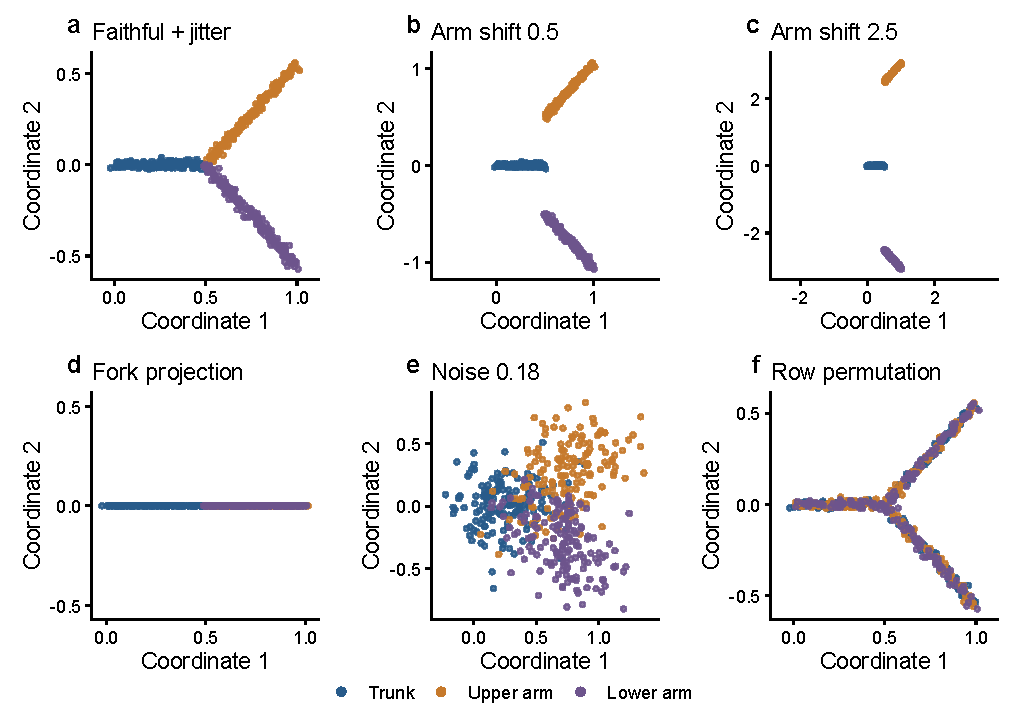
\includegraphics[width=\linewidth,height=0.64\textheight,keepaspectratio]{journal-figures/calibration_perturbations.pdf}
\caption{Matched-noise coordinate interventions for fixture seed 42. a, faithful candidate. b, opposing arm translations of 0.5. c, translations of 2.5. d, removal of the fork coordinate. e, additional Gaussian noise with standard deviation 0.18. f, permutation of candidate rows. Each view retains all 450 cells: 150 trunk cells and 150 in each arm. The shared colour key below the panels identifies the original branch labels, including after permutation. All damaged candidates start from the same faithful jitter realization, so the comparison does not remove baseline noise. Limits are chosen separately to resolve each coordinate configuration; aspect is equal, and absolute displacement must be read from the ticks rather than apparent panel span. Row permutation changes coordinate-to-cell correspondence while retaining label values and the marginal coordinate distribution. These are synthetic interventions, not observed biological trajectories.}
\label{fig:interventions}
\end{figure}
\FloatBarrier

\subsection{Reachability is a connectivity identity on a connected reference}
When the reference graph is connected, reachability equals the fraction of candidate pairs that occupy the same component. This equality held in all 322 applicable batteries (\figpanel{fig:reachability}{a}). It is a mathematical identity, not evidence that biological organization has been preserved. Five real-object cases with a disconnected reference lie outside that identity.

\begin{figure}[H]
\centering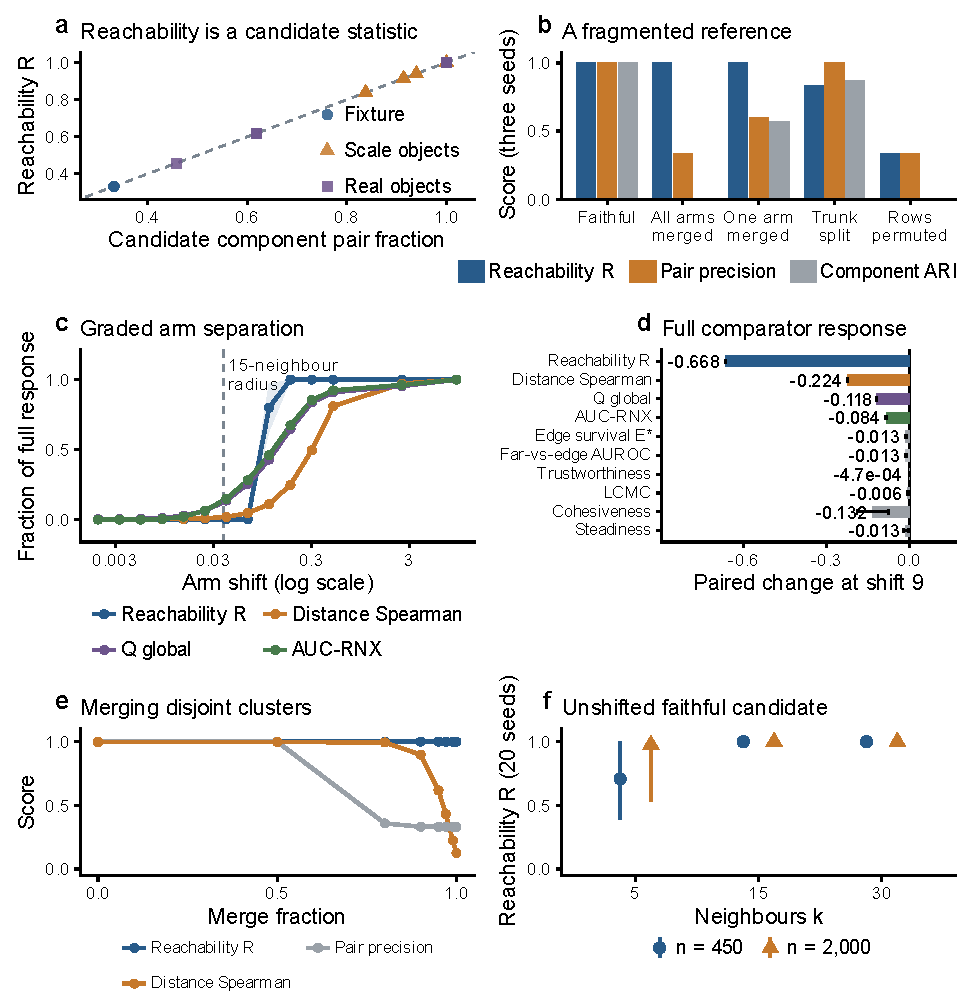
\includegraphics[width=\linewidth,height=0.74\textheight,keepaspectratio]{journal-figures/calibration_reachability.pdf}
\caption{What reachability measures. a, reachability against candidate component-pair fraction in the 322 connected-reference batteries; the dashed line is equality. b, a reference of three disjoint arms with five candidates (three-seed means): reachability ignores merging, which pair precision and component ARI detect. c, graded separation of the branching fixture ($n=450$, $k=15$, 20 seeds, independent candidate jitter); paired mean changes are divided by their mean response at shift 9. Ribbons show one seed standard deviation on that scale; the dashed line is the median reference 15th-neighbour distance. d, unnormalized paired mean changes at shift 9 for the complete displayed comparator set, with one-SD bars over the same seeds. e, merging three disjoint clusters by moving their centroids together, with seed-mean scores. f, reachability of the unshifted faithful candidate at three neighbour counts (points: seed means; bars: range over 20 seeds). Seed variability is fixture repeatability, not biological uncertainty.}
\label{fig:reachability}
\end{figure}
\FloatBarrier

A candidate that merges three reference-disconnected arms can retain reachability one while pair precision and component agreement fall (\figpanel{fig:reachability}{b}). In graded separation, global comparators responded at smaller tested displacements than reachability (\figpanel{fig:reachability}{c,d}). Reachability also ignored merging of disjoint clusters, and its baseline depended on neighborhood size (\figpanel{fig:reachability}{e,f}). It is therefore useful as a candidate-connectivity check within the stated regime; local, global and component diagnostics answer different questions.

\subsection{Sharpness-matched baselines change the coherence comparison}
Across twelve native allocation objects, unclipped coherence had median 0.812 and exceeded raw reference-fitted mixture responsibilities and random smooth maps (\figpanel{fig:coherence}{a}). Its descriptive association with one minus Geary's statistic was 0.993, consistent with a graph-smoothness ratio (\figpanel{fig:coherence}{b}). The raw mixture was sharper than the native probabilities. Matching its mean perplexity reduced the median native advantage to 0.029: native coherence was higher in eight objects and lower in all three lung objects (\figpanel{fig:coherence}{c}). No interval was calculated for this tempered comparison.

\begin{figure}[H]
\centering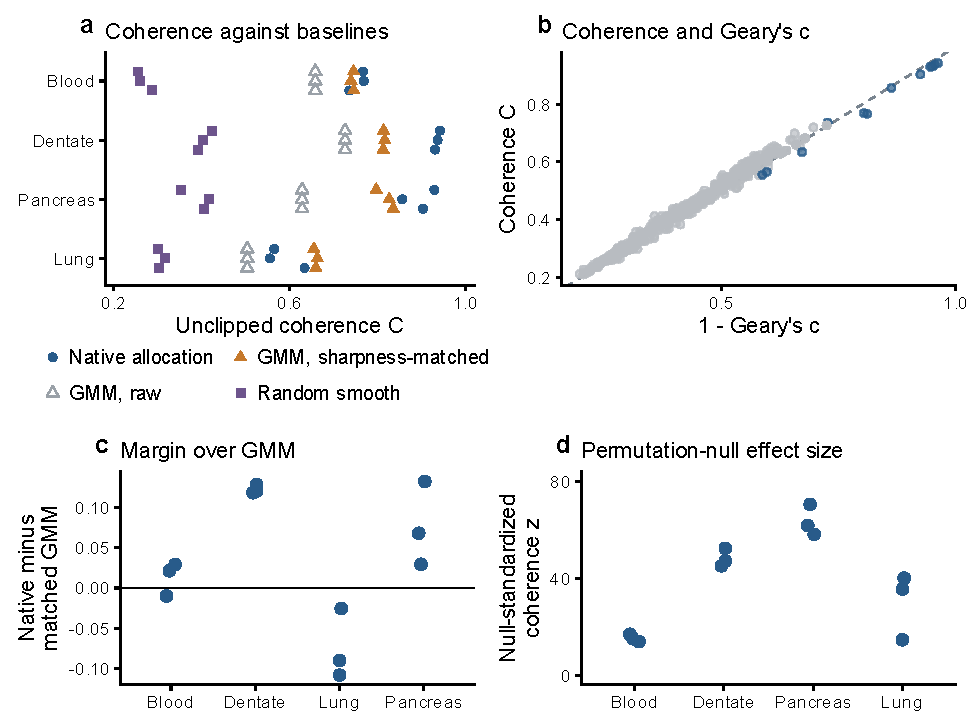
\includegraphics[width=\linewidth]{journal-figures/coherence_baselines.pdf}
\caption{Coherence against reference-aware baselines. a, unclipped coherence for twelve native objects, three stored seeds in each of four backgrounds, and three baselines: raw full-covariance Gaussian-mixture responsibilities on ten reference PCs, that mixture tempered to native mean perplexity, and the mean of 20 perplexity-matched random smooth maps. Vertical offsets separate stored seeds and have no quantitative meaning; horizontal position is coherence. The raw mixture is fitted to the reference, so its seeds have the same coherence. b, coherence against one minus multivariate Geary's $c$ on the same graph for native and raw-baseline allocations (native: blue; baselines: grey); the dashed line is equality. The reported association of 0.993 is restricted to the twelve native objects. c, native minus sharpness-matched mixture coherence by background; each point is one stored seed and the horizontal line is zero. d, native coherence standardized against its own 200-draw unclipped row-permutation null. Horizontal offsets separate stored seeds and have no quantitative meaning. No donor-level uncertainty or interval for the tempered mixture is implied.}
\label{fig:coherence}
\end{figure}
\FloatBarrier

Each object's own row-permutation null supplies a separate chance comparison (\figpanel{fig:coherence}{d}). The stored seeds are computational repeats, not independent biological samples. Exceeding an unmatched raw baseline or a permutation null does not establish useful allocation contrast.

\subsection{A favorable ratio can coexist with negligible absolute variation}
Coherence, probability dispersion and all-pair divergence describe different properties (\figpanel{fig:allocation}{a--c}). A near-uniform or constant allocation is guarded, while a sharp allocation can be coherent or incoherent depending on its correspondence to the reference. These operational checks do not certify biological usefulness.

\begin{figure}[H]
\centering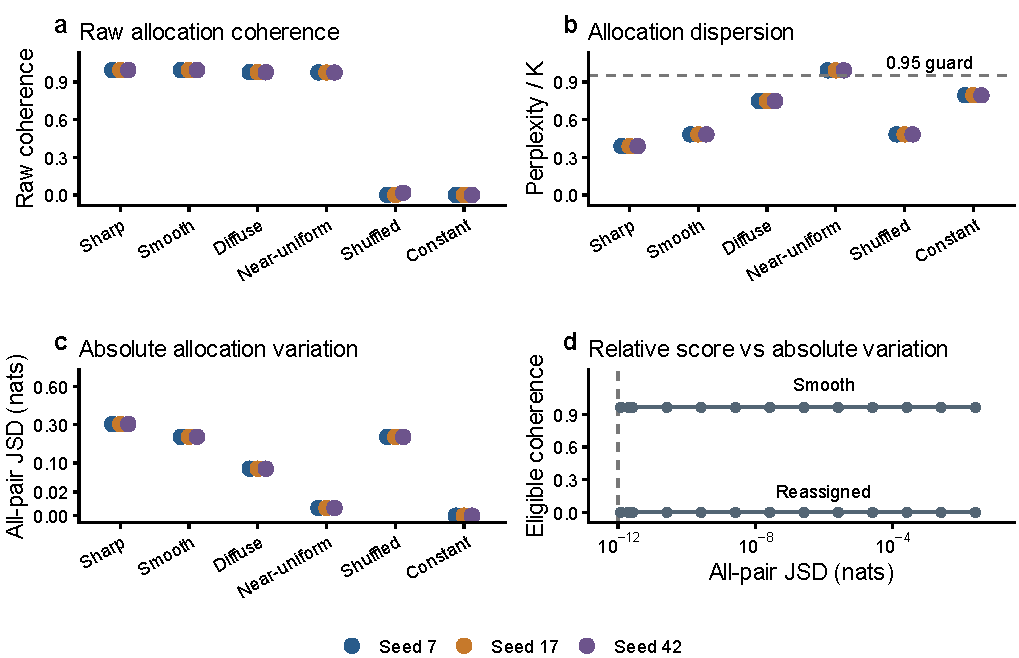
\includegraphics[width=\linewidth,height=0.64\textheight,keepaspectratio]{journal-figures/allocation_validity_guards.pdf}
\caption{Relative coherence, dispersion and absolute allocation variation. a, raw coherence for sharp, smooth, diffuse, near-uniform, shuffled and constant native controls. b, mean row perplexity divided by simplex dimension; the dashed 0.95 line marks the operational near-uniform guard. c, exact all-pair Jensen--Shannon divergence in nats on a square-root vertical axis. Coloured points and the shared seed key apply to a--c, retaining paired fixture seeds 7, 17 and 42 with horizontal offsets. Constant raw coherence is zero by guard convention. d, a separate independently validated 32-cell numerical fixture at $k=5$ varies tail mass in ten-coordinate probabilities $(1-\epsilon,\epsilon q_i)$ with smooth or bijectively reassigned nine-coordinate tails. Grey points show only numerically eligible cases; horizontal position is absolute all-pair divergence on a logarithmic axis, and the dashed line is the $10^{-12}$ denominator guard. Smooth coherence remains high across ten orders of absolute variation; reassignment reduces clipped coherence to zero. Guarded cases are retained in the numerical record but have no quotable ratio. The identity-explicit fixture implementation is distinct from the historical inventory scorer. Neither operational eligibility nor these synthetic replicates establishes biological usefulness or population-level uncertainty.}
\label{fig:allocation}
\end{figure}
\FloatBarrier

An independently validated numerical tail fixture gives the stronger counterexample (\figpanel{fig:allocation}{d}). Smooth coherence remained 0.964 when tail mass changed from one to $10^{-10}$, while all-pair divergence fell from $2.65\times10^{-2}$ to $2.65\times10^{-12}$ nats. Both examples passed the declared numerical guards. Reassigning the same rows changed coherence without changing the overall probability dispersion. A ratio therefore needs an absolute-variation measurement alongside its numerical eligibility rules.

\subsection{Candidate-specific chance correction changes representation rankings}
Increasing neighbor count raised both raw edge survival and its permutation expectation. Correcting for each candidate's own expectation reduced the scale effect (\figpanel{fig:chance}{a,b}).

\begin{figure}[H]
\centering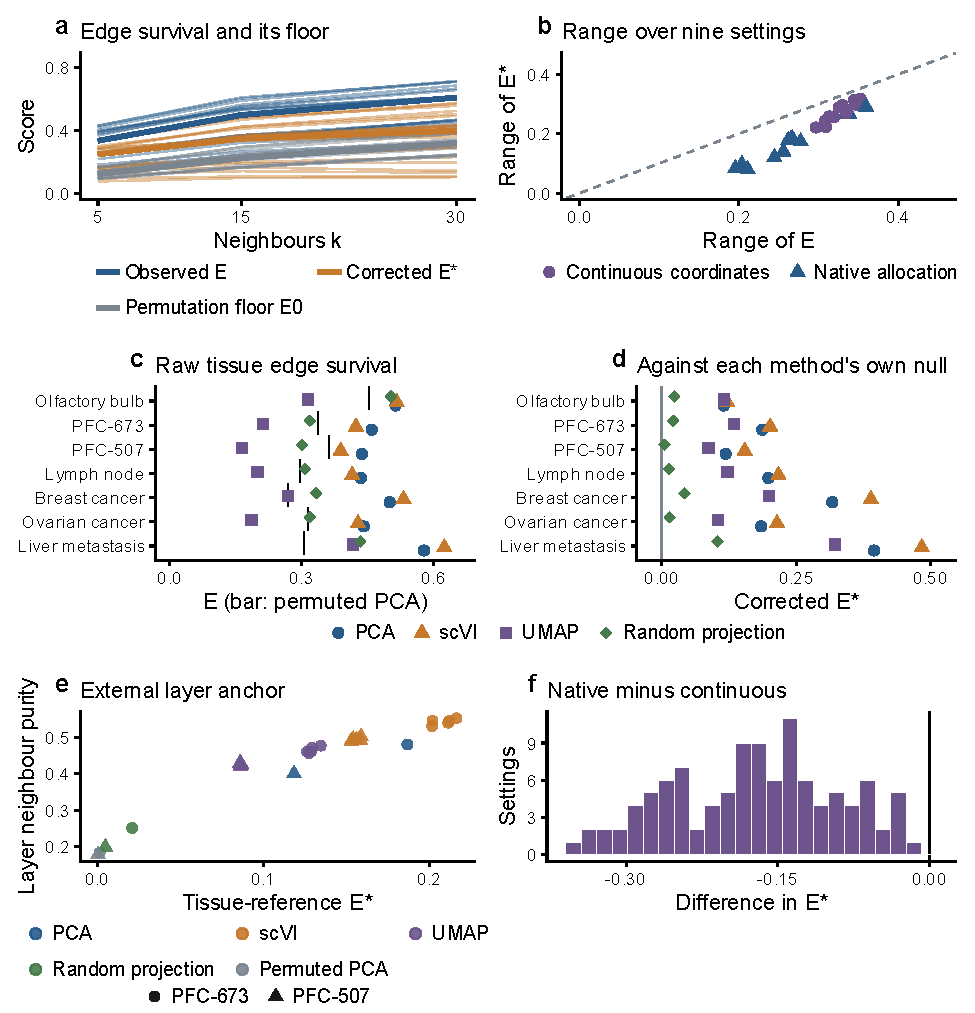
\includegraphics[width=\linewidth,height=0.74\textheight,keepaspectratio]{journal-figures/chance_correction.pdf}
\caption{Chance correction of edge survival. a, raw $E$, the 50-draw permutation mean $E_0$ and corrected $E^*$ against neighbour count for 24 scale objects at the 50-PC reference (thin lines: objects; thick lines: medians). b, within-object ranges over nine graph settings; the dashed line is equality. c, raw tissue-reference edge survival for regenerated candidates on seven sections; vertical bars mark permuted PCA. d, the same candidates corrected against their own 50-draw nulls. e, tissue-reference $E^*$ using exact candidate-pair expectations against candidate-neighbour cortical-layer purity on two prefrontal sections. Each section has thirteen plotted arrays: five scVI and five UMAP refits, plus PCA, random projection and permuted PCA; correlations exclude permuted PCA and use twelve arrays. f, native minus continuous corrected edge survival for all 108 matched settings. Arrays and settings are computational repeats, not independent biological units. Chance-correction panels use regenerated arrays, which reproduce the originally saved raw scores except for UMAP on one prefrontal section.}
\label{fig:chance}
\end{figure}
\FloatBarrier

Against tissue position, raw and corrected rankings differed because low-dimensional and higher-dimensional candidate graphs had different chance levels (\figpanel{fig:chance}{c,d}). The ordering changed in 11 of 15 object--reference comparisons. In the seven tissue sections, corrected scVI edge survival matched or exceeded PCA, whereas raw scores placed PCA higher on four. These are conditional computational comparisons, not a ranking against biological ground truth.

The relationship with cortical-layer purity was descriptive in two sections, with repeated representation seeds rather than independent donors (\figpanel{fig:chance}{e}). Native-versus-continuous contrasts retained all matched settings (\figpanel{fig:chance}{f}). Tie sensitivities and alternative references did not justify universal conclusions about metrics or representations. Tissue and expression coordinate views, complete chance expectations and implementation-specific calibration are provided in the supplement.

The primary result is that chance expectations and sharpness-matched baselines can change conclusions drawn from raw scores. The implementation agreement validates arithmetic within the declared inputs and conventions. It does not validate a biological reference, supply missing donor replication or reconstruct the historical external calibration driver.

































\section{Discussion}
The experiments support a conditional interpretation of geometric fidelity, and they show that the condition has to include the chance level of each score. Matching the starting noise removed an apparent local-score improvement under arm separation, and direct execution of the official trajectory API gave a strong shatter response that the local root-distance surrogate did not reproduce; those corrections address experimental confounding and implementation misidentification.

The second correction reverses several comparisons. Scored against its own permutation, UMAP retained tissue neighbourhoods above chance in edge survival on every section, and scVI matched or exceeded PCA on all seven fixed arrays, whereas raw edge survival placed PCA higher on four of the seven.

The same reasoning applies to allocation coherence. Native allocations exceeded random smooth and raw mixture baselines everywhere, but a mixture fitted to the reference and tempered to the same sharpness came close and exceeded them in lung.

Exact coherence improves one narrower aspect of reproducibility. Its denominator is a property of all distinct allocation pairs and therefore does not depend on which row positions happened to enter a random sample.

The stored-data census illustrates the importance of that eligibility denominator. Continuous coordinates, native allocations, guarded allocations, duplicate files, and repeated checkpoints all occur in the available collection.

Several design choices remain limitations of this measurement study. The archived calibration used identical reference and faithful noise draws; the graded calibration decoupled them and added three topologies without changing the conclusions, but all fixtures remain planar and noiseless in expression.

The practical implication is to make evaluation records more explicit. A reusable result should retain matched row identities, the reference construction, graph settings, the semantic type of the candidate, implementation versions, and unavailable or guarded outputs.

Biological validity needs an external target of its own. Count simulators such as Splatter~\cite{zappia2017splatter} and dynamic simulators such as dyngen~\cite{cannoodt2021dyngen} would extend the planar fixtures to realistic expression with known topology, and clonal lineage measurements~\cite{weinreb2020lineage} could test whether a corrected geometric score predicts observed fate.

\section{Methods}
\subsection{Measurement workflow and analysis objects}

The coordinate input is a finite matrix $Z\in\mathbb R^{n\times q}$ paired row-for-row with a reference $X\in\mathbb R^{n\times d}$. The allocation pathway additionally requires model-declared probabilities $P\in\Delta^{K-1}$ for each cell; numeric normalization alone cannot supply that interpretation. Graph scores, allocation eligibility, dispersion and null comparisons remain separate outputs. No combined biological-success score is constructed. Preprocessing and the chosen reference define the question being asked, as they do elsewhere in single-cell analysis~\cite{luecken2019practices}. We call the implementation that produced the stored results the archived scorer; later sections compare it with an exact, identity-explicit reimplementation.



\subsection{Reference-anchored geometry}

Let $X=(x_i)_{i=1}^n$ be the reference and $Z=(z_i)_{i=1}^n$ the candidate, with the same cell identity in each row. On each space we construct the undirected union of a Euclidean $k$-nearest-neighbour graph, using $k=15$. Let $h_X(i,j)$ and $h_Z(i,j)$ denote unweighted shortest-path distances, with infinity for disconnected pairs. Let $\mathcal P_X=\{(i,j):i<j,\ h_X(i,j)<\infty\}$ and let $E_X$ be the undirected reference edges. Reachability and edge survival are
\begin{align}
 R(X,Z)&=\frac{1}{|\mathcal P_X|}\sum_{(i,j)\in\mathcal P_X}\mathbf 1[h_Z(i,j)<\infty],\label{eq:reachability}\\
 E(X,Z)&=\frac{1}{|E_X|}\sum_{(i,j)\in E_X}\frac{1}{h_Z(i,j)},\qquad 1/\infty=0.
\end{align}
The first counts connected pairs; the second measures local adjacency distortion. A small number of severed junction edges can disconnect many pairs. Conversely, a connected but randomly reordered candidate can have $R=1$, so $R$ alone is not a quality score. Neighbours use Euclidean distance and the union rather than intersection of directed neighbour lists, with $k'=\min(k,n-1)$ for a positive integer $k$ (the archived constructor additionally raises $k<1$ to one). Graph edges carry unit weight. Each unordered pair or edge enters its denominator once; the score formulas exclude self-pairs. The archived neighbour constructor drops the first returned rank, assuming it is the query itself. Exact duplicates can violate this assumption; the tie stress test below therefore delimits this implementation. Nonfinite inputs and reference populations with fewer than ten connected pairs are rejected instead of receiving a favourable score. The identity-explicit reimplementation described below reports no graph score when all rows of the reference or of the candidate are identical; the archived scorer still constructs a union nearest-neighbour graph on such input and can emit self-loops.

For separation survival, the reference far set $F_X$ contains the finite reference pairs whose hop distance is at least the 90th percentile $q_{0.9}$ of the finite values of $h_X$ (interpolated linearly at rank $1+0.9(N-1)$ among the $N$ sorted finite values); separation is withheld when $F_X$ has fewer than ten pairs. Let $m_Z$ be the median of the finite values of $h_Z$, the mean of the two central values when their number is even. We define
\begin{equation}
 S(X,Z)=\frac{1}{|F_X|}\sum_{(i,j)\in F_X}\mathbf 1[h_Z(i,j)\geq m_Z].
\end{equation}
Disconnected candidate pairs count as separated; the union graph of two or more rows always contains an edge, so the candidate always has a finite hop. This convention is complementary to reachability, but the candidate-dependent threshold also limits interpretation: $S$ is not an absolute distance-preservation measure. Graph construction, tied distances, $k$, and the chosen reference can change the answer. The baseline setting is $k=15$ with a 50-component reference. The additional sensitivity experiment varies $k$ and the retained reference dimension explicitly, over a finite grid described below.



\subsection{Chance expectations and tie-aware separation}

Uniformly permuting candidate rows while fixing the reference maps each distinct reference pair to a uniformly selected candidate pair. If the candidate graph is invariant to row relabelling, the exact expectations are
\begin{equation}
 E_0^{\rm exact}=\frac{1}{\binom n2}\sum_{i<j}\frac{1}{h_Z(i,j)},\qquad
 S_0^{\rm exact}=\frac{1}{\binom n2}\sum_{i<j}\mathbf 1[h_Z(i,j)\geq m_Z].
\end{equation}
Disconnected distances retain the conventions above. The scale and diversity chance-correction analyses use the means of 50 row-permutation draws, $E_0^{\rm MC}$ and $S_0^{\rm MC}$; the graded calibration and representation refits use the exact expectations. With the corresponding null denoted $E_0,S_0$, the corrected scores are
\begin{equation}
 E^*=\frac{E-E_0}{1-E_0},\qquad S^*=\frac{S-S_0}{1-S_0}.\label{eq:corrected}
\end{equation}
Correction is undefined when its null is one; such cases are not replaced by zero. In the 216 scale batteries, the largest Monte Carlo--exact discrepancies were 0.0014 for $E_0$ and 0.0054 for $S_0$. Candidate cutoff ties were absent in those arrays and in the regenerated diversity candidates. This check does not resolve ties in lattice-like tissue references under the archived neighbour constructor.

Integer-hop ties also affect the candidate-median threshold. The complementary far-versus-edge AUROC compares every reference far pair $f\in F_X$ with every reference edge $e\in E_X$:
\begin{equation}
 A_{FE}=\frac{1}{|F_X||E_X|}\sum_{f\in F_X}\sum_{e\in E_X}
 \left\{\mathbf 1[h_Z(f)>h_Z(e)]+\tfrac12\mathbf 1[h_Z(f)=h_Z(e)]\right\}.
\end{equation}
Infinite distances receive the highest tied rank, including half credit when both are infinite. The permutation expectation is 0.5. This is tie-aware rather than tie-free, and it does not by itself penalize all forms of fragmentation.



\subsection{Exact coherence and applicability}

Allocation coherence requires a native allocation matrix $P$ with rows $p_i\in\Delta^{K-1}$ representing probabilities over the model's allocation coordinates. The Jensen--Shannon divergence~\cite{lin1991divergence} is computed in natural-log units after the implementation's fixed $10^{-12}$ clipping and row renormalization. Define
\begin{align}
 D_E &= |E_X|^{-1}\sum_{(i,j)\in E_X}\operatorname{JSD}(p_i,p_j),\\
 D_{\rm all} &= {\binom n2}^{-1}\sum_{i<j}\operatorname{JSD}(p_i,p_j),\\
 C_{\rm raw} &= \left[1-D_E/D_{\rm all}\right]_0^1.
\end{align}
For two allocation rows, with $m=(p+q)/2$,
\begin{equation}
 \operatorname{JSD}(p,q)=\frac12\sum_jp_j\log\frac{p_j}{m_j}
                         +\frac12\sum_jq_j\log\frac{q_j}{m_j}.
\end{equation}
The coherence denominator uses every unordered distinct pair in $D_{\rm all}$. The historical implementation sampled positional pairs using a fixed seed. Jointly reordering reference and allocation rows therefore changed the sampled denominator even though the scientific object was unchanged. Exact summation removes this sampling dependence, up to floating-point accumulation, at $O(n^2K)$ arithmetic cost. The implementation uses bounded row-block memory for the denominator; all-pairs graph distances still require quadratic storage. Unit tests compare the denominator with independently enumerated SciPy Jensen--Shannon distances and test joint row reordering.

On the clipped and renormalized rows, the normalized mean row perplexity is
\begin{equation}
 \Pi(P)=\frac{1}{nK}\sum_i\exp\!\left[-\sum_jp_{ij}\log p_{ij}\right].
\end{equation}
A denominator at or below $10^{-12}$ marks the allocation degenerate, and $\Pi(P)>0.95$ marks it near-uniform. Neither yields a quotable coherence value; the degenerate raw diagnostic is set to zero by convention. A constant uniform matrix satisfies both conditions and is classed as degenerate. The thresholds are declared operational guards, not estimated biological decision boundaries. Raw diagnostics remain available for auditing.

Continuous Gaussian coordinates are classed as non-native. A softmax of these coordinates is tabulated separately from native coherence; its dimension is the number of latent coordinates, which is 10 for the stored mixture-regularized representations, not their mixture truncation of 50. That transformation is not a posterior responsibility matrix and cannot support allocation claims. The inventory and all reported re-scores declare allocation semantics explicitly instead of inferring them from the numerical values.



\subsection{Calibration, baselines and statistical scope}
Controlled coordinate interventions used matched initial noise so that denoising could not masquerade as preservation of geometry. The exact diagnostic implementation was checked against an independently written scorer. Chance expectations were candidate-specific, and allocation baselines matched both native probability semantics and sharpness. Synthetic seeds characterized computational repeatability. Stored representations and tissue sections were computational objects, not independent donors, and correlations with annotations remained descriptive. The full fixture grids, allocation eligibility rules, component identities, baseline construction and uncertainty procedures are preserved in the Supplementary Methods. The earlier external calibration driver is not redistributed; supplied saved-calibration replay is narrower than a complete rerun of that driver.

\subsection{Ethics and computational assistance}
This study reanalyzed synthetic fixtures and previously published public single-cell and spatial transcriptomics datasets. No new participants were recruited and no human or animal specimens were collected. Ethical oversight and consent for the original measurements are described by the source studies; no new institutional approval or exemption is claimed here.

OpenAI Codex (OpenAI) assisted with code development, execution and checking of computational analyses, suggestions for analytical and methodological checks, manuscript drafting and restructuring, extensive language editing, and LaTeX and figure preparation. Reported numerical results were checked against saved outputs, and scripts and document builds were verified using the procedures described in this article and its Supplementary Information. AI-assisted critique and verification are preparation aids and do not constitute independent human peer review. The author directed the work and retains responsibility for the study design, data provenance, choice of analyses, scientific interpretation and final manuscript. No generative images were used as research data.

\section{Declarations}

\section*{Data Availability}
The accompanying source bundle contains this revision's code, figure sources, saved score tables and the distributed candidate and reference arrays. The public repository is \url{https://github.com/PeterPonyu/reference-anchored-geometry}. The earlier software release is archived at \url{https://doi.org/10.5281/zenodo.22914409}; that immutable archive does not contain the present revision. The frozen analysis release is archived at \url{https://doi.org/10.5281/zenodo.23308078}. The bundle includes synthetic calibration arrays, 24 matched representation and reference arrays, seven tissue-section representations and one blood-sample representation, numerical tests and reproduction instructions. Public count matrices, complete expression caches, remaining historical latent files and the historical multi-library calibration driver are not redistributed; their source and reproduction limits are stated in the guide. Author-owned software is MIT licensed; author-owned research content is CC BY 4.0; third-party materials retain their original terms.

\section*{Code availability}
Analysis code, the identity-explicit scorer, saved calibration inputs and numerical validation are available at \url{https://github.com/PeterPonyu/reference-anchored-geometry} and archived at software DOI \url{https://doi.org/10.5281/zenodo.23308078}. The reproduction guide distinguishes saved-array analyses from steps requiring source count matrices or the historical calibration driver.

\noindent\textbf{Funding}\par\nobreak

This research received no external funding.



\section*{Additional Information}
The author declares no competing interests.

{\footnotesize\raggedright\setlength{\bibsep}{1pt}\setlength{\emergencystretch}{3em}
The software archive is the frozen computational evidence. The present submission revision and its editable document sources are separately versioned in the same repository.

\bibliographystyle{naturemag}
\bibliography{references}}

\section*{Author contributions}
Zeyu Fu is the sole author and was responsible for all aspects of the study and manuscript. Zeyu Fu is the corresponding contact for this manuscript.

\end{document}
